\documentclass[tikz,border=3pt]{standalone}
\usepackage[utf8]{inputenc}
\usepackage[T1]{fontenc}
\usepackage{lmodern}
\renewcommand{\familydefault}{\sfdefault}
\usepackage{sansmath}\sansmath
\usepackage{chemfig}
\usepackage{pgfplots}\pgfplotsset{compat=1.18,/pgf/number format/use comma,/pgf/number format/1000 sep={.}}
\usetikzlibrary{arrows.meta,calc,positioning,decorations.pathmorphing,patterns}
% paleta del sitio
\definecolor{nar}{HTML}{E8680C}\definecolor{narc}{HTML}{FFB35C}\definecolor{hielo}{HTML}{FFF3E8}
\definecolor{tinta}{HTML}{1D1D1F}\definecolor{gris}{HTML}{6E6E73}\definecolor{lila}{HTML}{7C5CF0}
\definecolor{azul}{HTML}{2F6FD6}\definecolor{menta}{HTML}{17A673}\definecolor{coral}{HTML}{E8342A}
\begin{document}
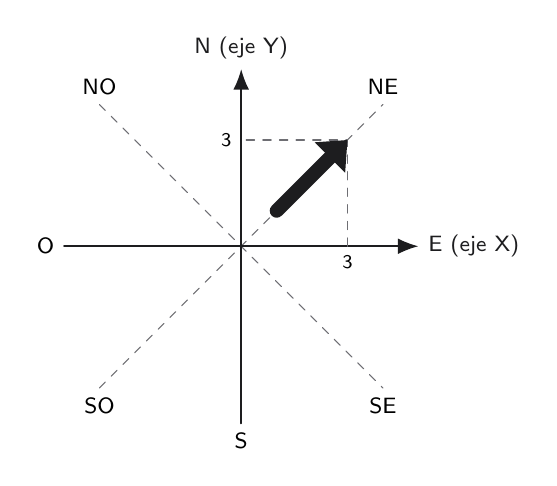
\begin{tikzpicture}[font=\small,x=0.45cm,y=0.45cm,line cap=round,line join=round,step={(1,1)}]
\draw[gris,dashed] (-4,-4)--(4,4); \draw[gris,dashed] (-4,4)--(4,-4);
\draw[-{Latex[length=2.6mm,width=2mm]},tinta,semithick] (-5,0)--(5,0) node[right,font=\footnotesize] {E (eje X)};
\draw[-{Latex[length=2.6mm,width=2mm]},tinta,semithick] (0,-5)--(0,5) node[above,font=\footnotesize] {N (eje Y)};
\node[left,font=\footnotesize] at (-5,0) {O}; \node[below,font=\footnotesize] at (0,-5) {S};
\node[above,font=\footnotesize] at (4,4) {NE}; \node[above,font=\footnotesize] at (-4,4) {NO};
\node[below,font=\footnotesize] at (4,-4) {SE}; \node[below,font=\footnotesize] at (-4,-4) {SO};
\draw[gris,dashed] (3,0)--(3,3)--(0,3);
\node[below,font=\scriptsize] at (3,0) {3}; \node[left,font=\scriptsize] at (0,3) {3};
\draw[line width=5pt,tinta,-{Triangle[length=9pt,width=15pt]}] (1,1)--(3,3);
\end{tikzpicture}
\end{document}
